\chapter{Riemann Sums}

When taking a left Riemann sum, the height of the rectangle is determined by the value of the function at the lower (left-most) $x$-value. See figure \ref{fig:leftriemann}. Based on the graph, do you think a left Riemann sum overestimates or underestimates the area under the curve?

%fixme rectangles show in overleaf but not build%

\begin{figure}
    \centering
    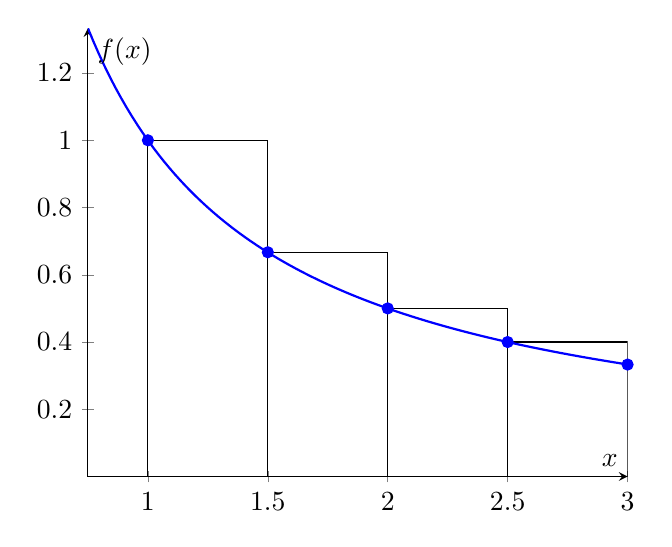
\begin{tikzpicture}
        \begin{axis}[axis lines = center, xmin=0.75, xmax=3, ymin=0, xlabel=$x$, ylabel=$f(x)$]
            \draw (1,0) rectangle (1.5,1);
            \draw (1.5,0) rectangle (2, 0.667);
            \draw (2,0) rectangle (2.5, 0.5);
            \draw (2.5,0) rectangle (3, 0.4);
            \addplot[blue, thick, samples=100, domain=0.75:3]{1/x};
            \addplot[mark=*, blue, only marks]coordinates{(1,1) (1.5,0.667) (2, 0.5) (2.5,.4) (3,0.333)};
        \end{axis}
    \end{tikzpicture}
    \caption{Left Riemann sum of $f(x)=\frac{1}{x}$}
    \label{fig:leftriemann}
\end{figure}

A right Riemann sum uses the right-most value of $f(x)$ to determine the height of the rectangle. As you can see in figure \ref{fig:rightriemann}, right Riemann sums underestimate the area under concave up curves. 

\begin{figure}
    \centering
    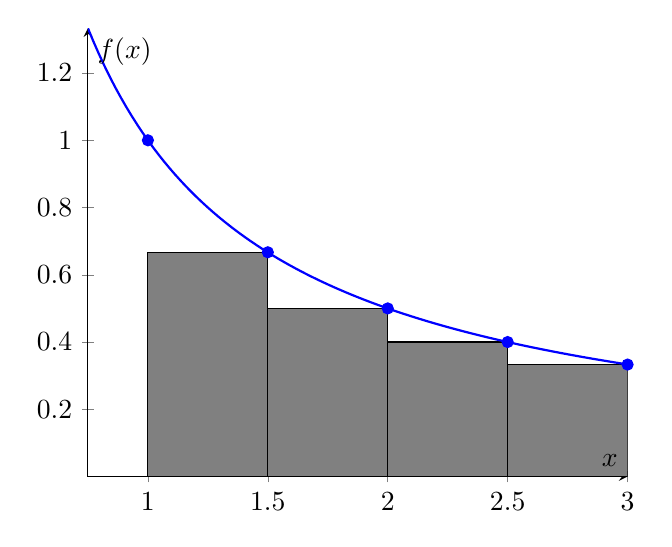
\begin{tikzpicture}
        \begin{axis}[axis lines = center, xmin=0.75, xmax=3, ymin=0, xlabel=$x$, ylabel=$f(x)$]
            \filldraw[fill=gray] (1,0) rectangle (1.5,0.667);
            \filldraw[fill=gray] (1.5,0) rectangle (2, 0.5);
            \filldraw[fill=gray] (2,0) rectangle (2.5, 0.4);
            \filldraw[fill=gray] (2.5,0) rectangle (3, 0.333);
            \addplot[blue, thick, samples=100, domain=0.75:3]{1/x};
            \addplot[mark=*, blue, only marks]coordinates{(1,1) (1.5,0.667) (2, 0.5) (2.5,.4) (3,0.333)};
        \end{axis}
    \end{tikzpicture}
    \caption{Right Riemann sum of $f(x)=\frac{1}{x}$}
    \label{fig:rightriemann}
\end{figure}

A midpoint Riemann sum uses the value of $f(x)$ at the midpoint of the division to determine the height of the rectangle, as shown in figure \ref{fig:midriemann}. 

\begin{figure}
    \centering
    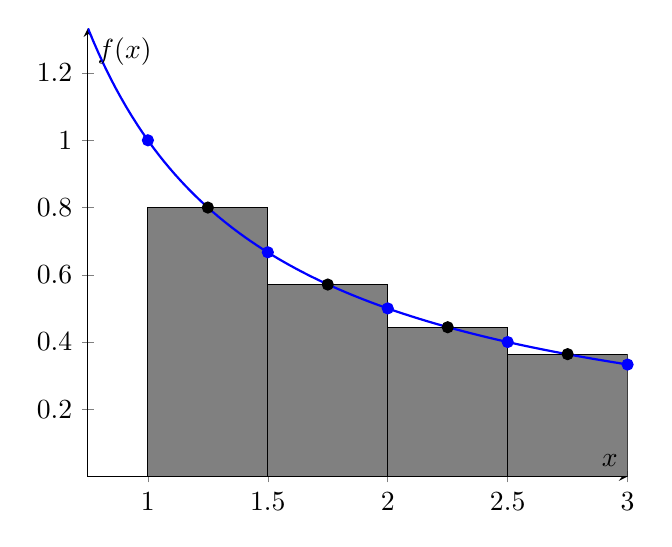
\begin{tikzpicture}
        \begin{axis}[axis lines = center, xmin=0.75, xmax=3, ymin=0, xlabel=$x$, ylabel=$f(x)$]
            \filldraw[fill=gray] (1,0) rectangle (1.5,0.8);
            \filldraw[fill=gray] (1.5,0) rectangle (2, 0.571);
            \filldraw[fill=gray] (2,0) rectangle (2.5, 0.444);
            \filldraw[fill=gray] (2.5,0) rectangle (3, 0.364);
            \addplot[blue, thick, samples=100, domain=0.75:3]{1/x};
            \addplot[mark=*, blue, only marks]coordinates{(1,1) (1.5,0.667) (2, 0.5) (2.5,.4) (3,0.333)};
            \addplot[mark=*, black, only marks]coordinates{(1.25,0.8) (1.75,0.571) (2.25, 0.444) (2.75,.364)};
        \end{axis}
    \end{tikzpicture}
    \caption{Midpoint Riemann sum of $f(x)=\frac{1}{x}$}
    \label{fig:midriemann}
\end{figure}

\begin{Exercise}[label=rsum1]
	\begin{center}
		\begin{tabular}{c|c|c|c|c}
			t (hours) & 4 & 7 & 12 & 15\\
			R(t) (L/hr) & 6.5 & 6.2 & 5.9 & 5.6\\
		\end{tabular}
	\end{center}
	A tank contains 50 liters of water after 4 hours of filling. Water is being added to the tank at rate $R(t)$. The value of $R(t)$ at select times is shown in the table. Using a right Riemann sum, estimate the amount of water in the tank after 15 hours of filling. 
\end{Exercise}

\begin{Answer}[ref=rsum1]
	The volume of water will be the amount of water at 4 hours (50 liters) plus the area under the graph of $R(t)$ from $t=4$ to $t=15$. We will estimate this area with a right Riemann sum. The approximate volume added from $t=4$ to $t=7$ is $(7-4)*(6.2) = 18.6$ liters. The approximate volume added from $t=7$ to $t=12$ is $(12-7)*(5.9)=29.5$ liters. The approximate volume added from $t=12$ to $t=15$ is $(15-12)*(5.6) = 16.8$ liters. Therefore, the approximate total volume of water in the tank at $t=15$ is $50 + 18.6 + 29.5 + 16.8 = 114.9$ liters. 
\end{Answer}